\section{Roadmap}

\subsection{Operation Model And Procedure}
The BottAll will be entirely designed and improved in the R\&D of our society. Once it is finally finished, the project of the main pieces will be sent to partner companies in order to be manufactured. We will strictly work together with them in order to provide the best product with the best peculiarities and to solve future possible issues.\\
Suppliers will be sent their product directly to our facility where the product will be assembled by our workers. In particular, the electronic circuit will be integrated in the bottle.\\
After the assembling part will be completed, the product will be packed and stored in the warehouse where it will stay until sold. Our purpose is to keep a well provided warehouse in order to have short time between order and delivery. The product will be ready for shipment.\\
BottAll will be sold mainly through our online shop were the costumer can find specs of the bottle and about our society. However, the website is not the only place people can find us. We will also be present in some shops such as Zara Home and Maison du Monde. The idea is to offer our product as a great new idea for an original present.
\begin{figure}[H]
\centering
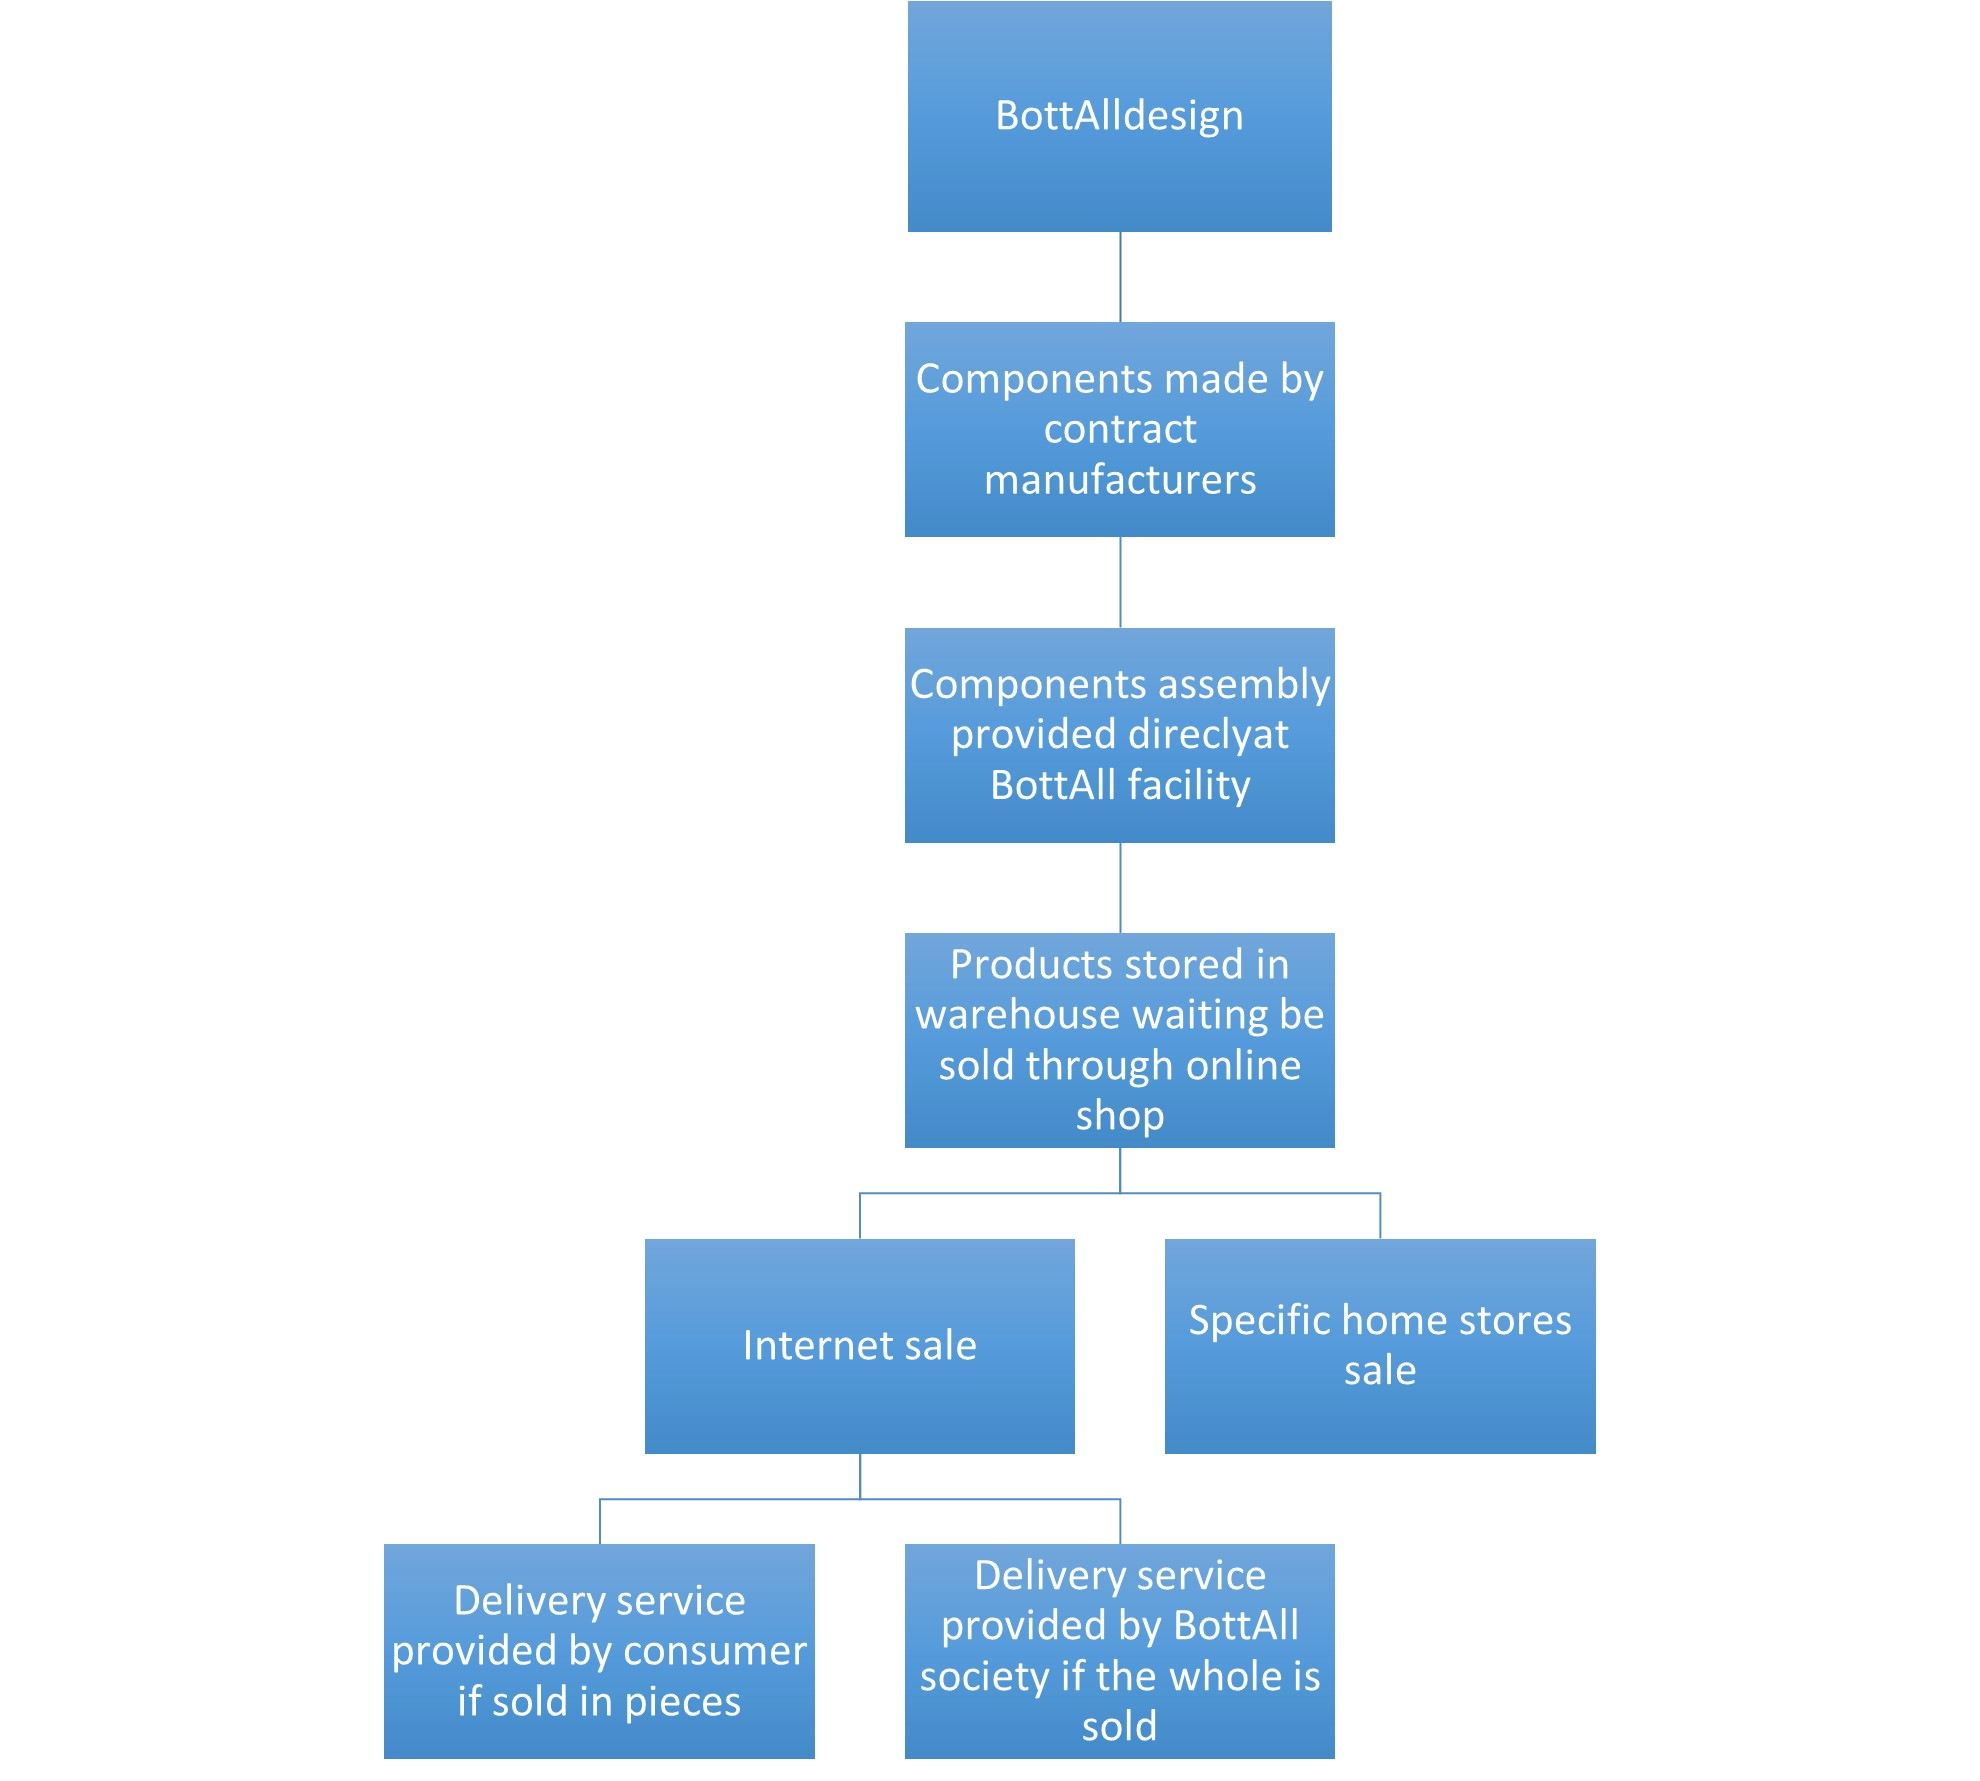
\includegraphics[width=0.8\textwidth]{images/flow_diagram.jpg}
\caption{OPERATION FLOW DIAGRAM}
\end{figure}

\subsection{Business Location}
The company will arise in Bologna. The choice for the location is not random. We decided that this city is the perfect place for make our society grow. As a matter of fact, Bologna is in the middle between the north and the south of the Italy and in addition it is not far from the borders with Europe. These features mean that we will be close both to suppliers and customers and we will have easy access to the main transportation roads.
Bologna is known also for its well rated University. This condition is perfect for the growth of our company because a qualified labor force will be needed and so there is nothing better than new graduate students from one of the best University in Italy.
Finally, even if Bologna is a great industrial node for the Italian economy it is some way cheaper than other big industrial poles such as Milan for example, so it is the right place for a small company to prosper.
\begin{figure}[H]
\centering
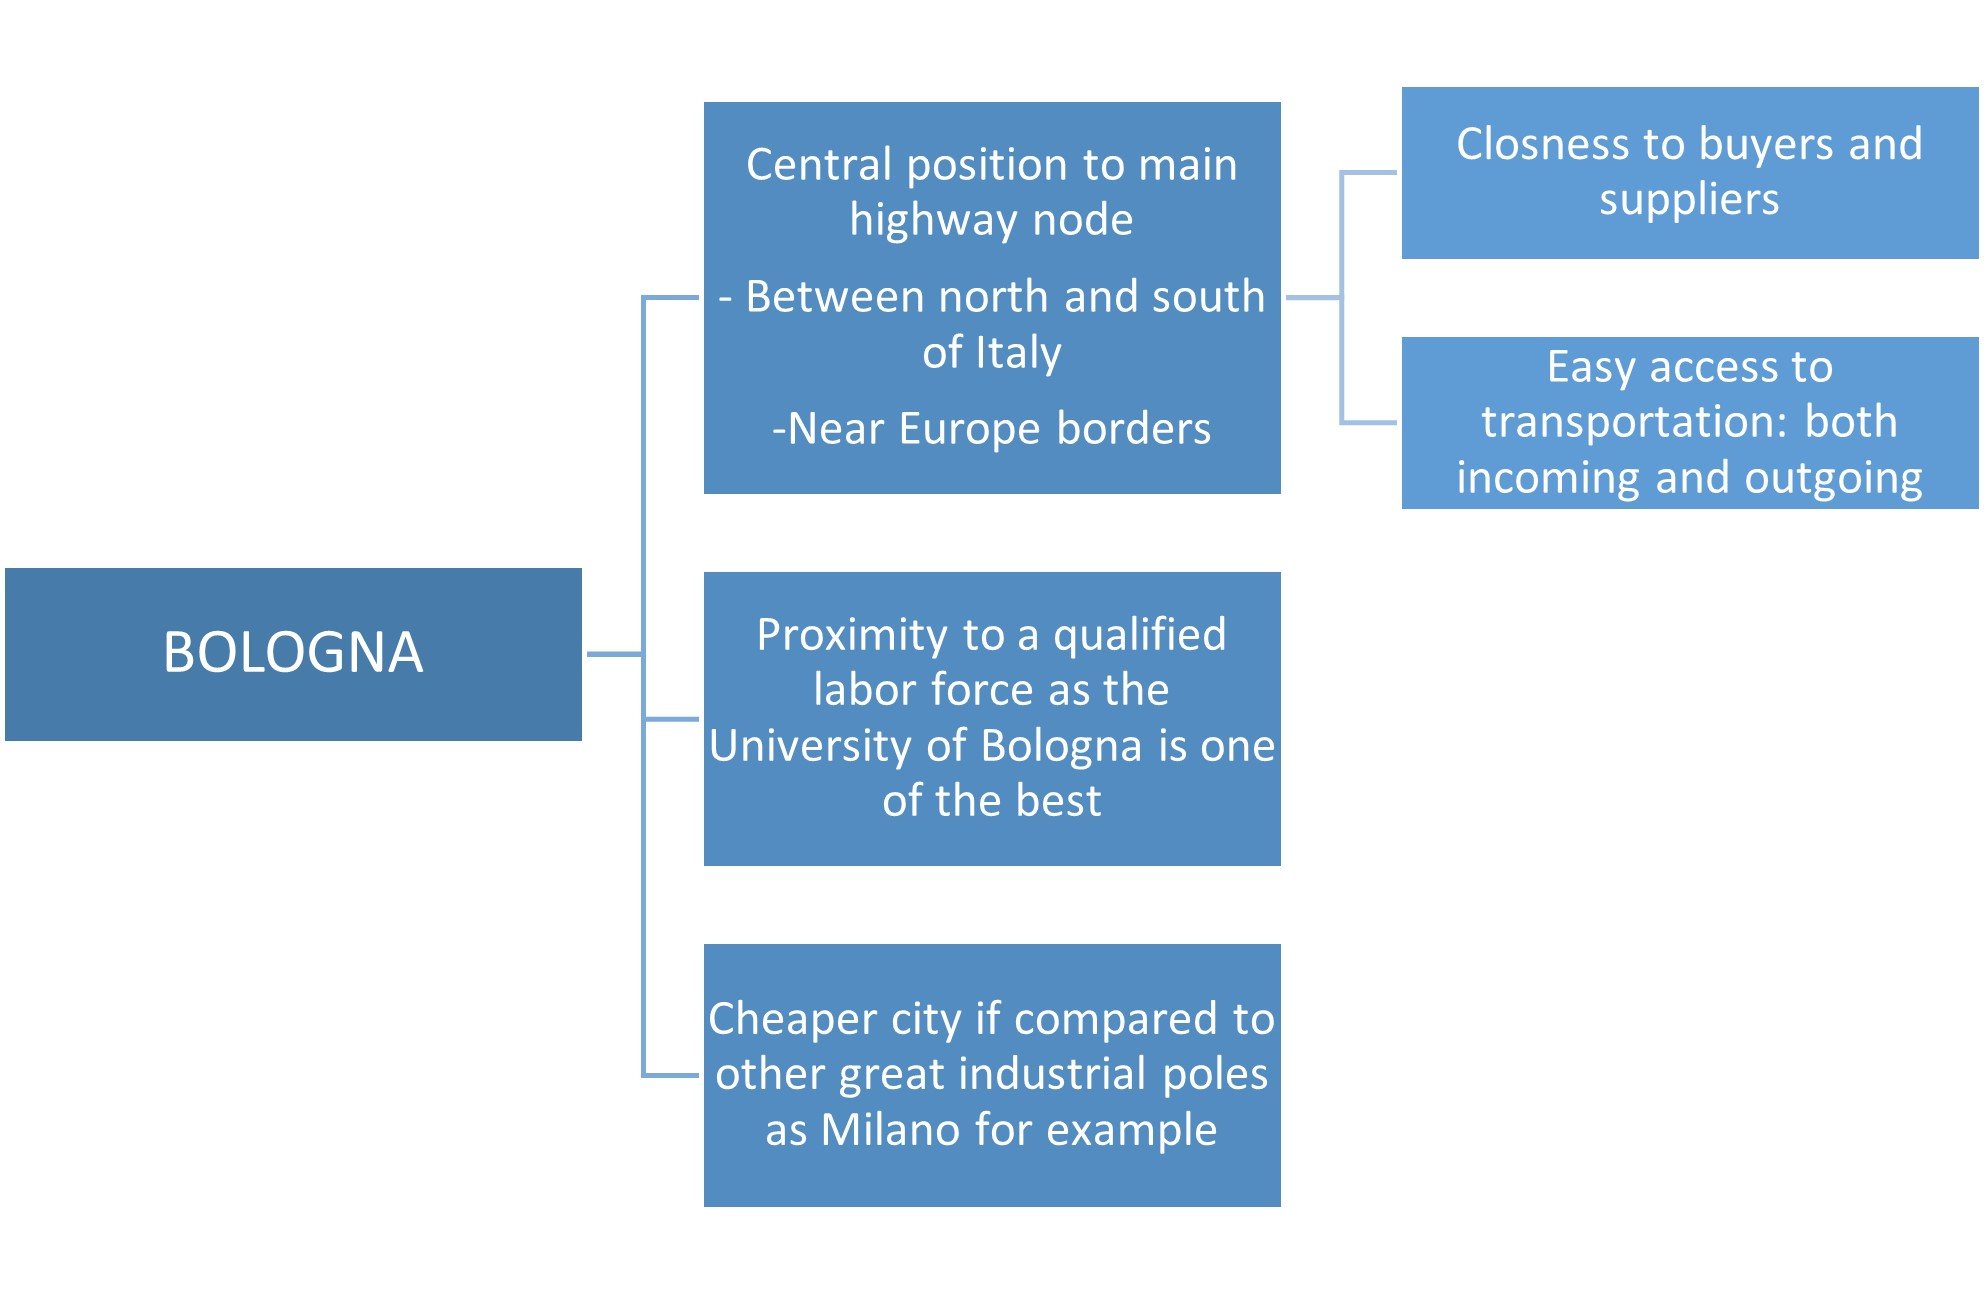
\includegraphics[width=1\textwidth]{images/Location.jpg}
\caption{Business Location}
\end{figure}

\subsection{Facilities And Equipment}
For the first step of the company, a small facility will be needed. Of course, it would be too expensive to buy it, so initially it will be leased. 
The facility will be split in three main sections. The first will serve as a work-space where our workers can assemble the final product and update the software needed by the bottle. In this section, the basic machines useful for the production will be also put such as a soldering station or some computers.
The second section will be devoted to offices for business management, research and development, and for the programming team focused on the software for the BottAll and for the website.
The last part, and of course the biggest, will serve as a warehouse were the product will be stored at the end of the production and where basic pieces coming from suppliers will stay until the assembling.
\begin{figure}[H]
\centering
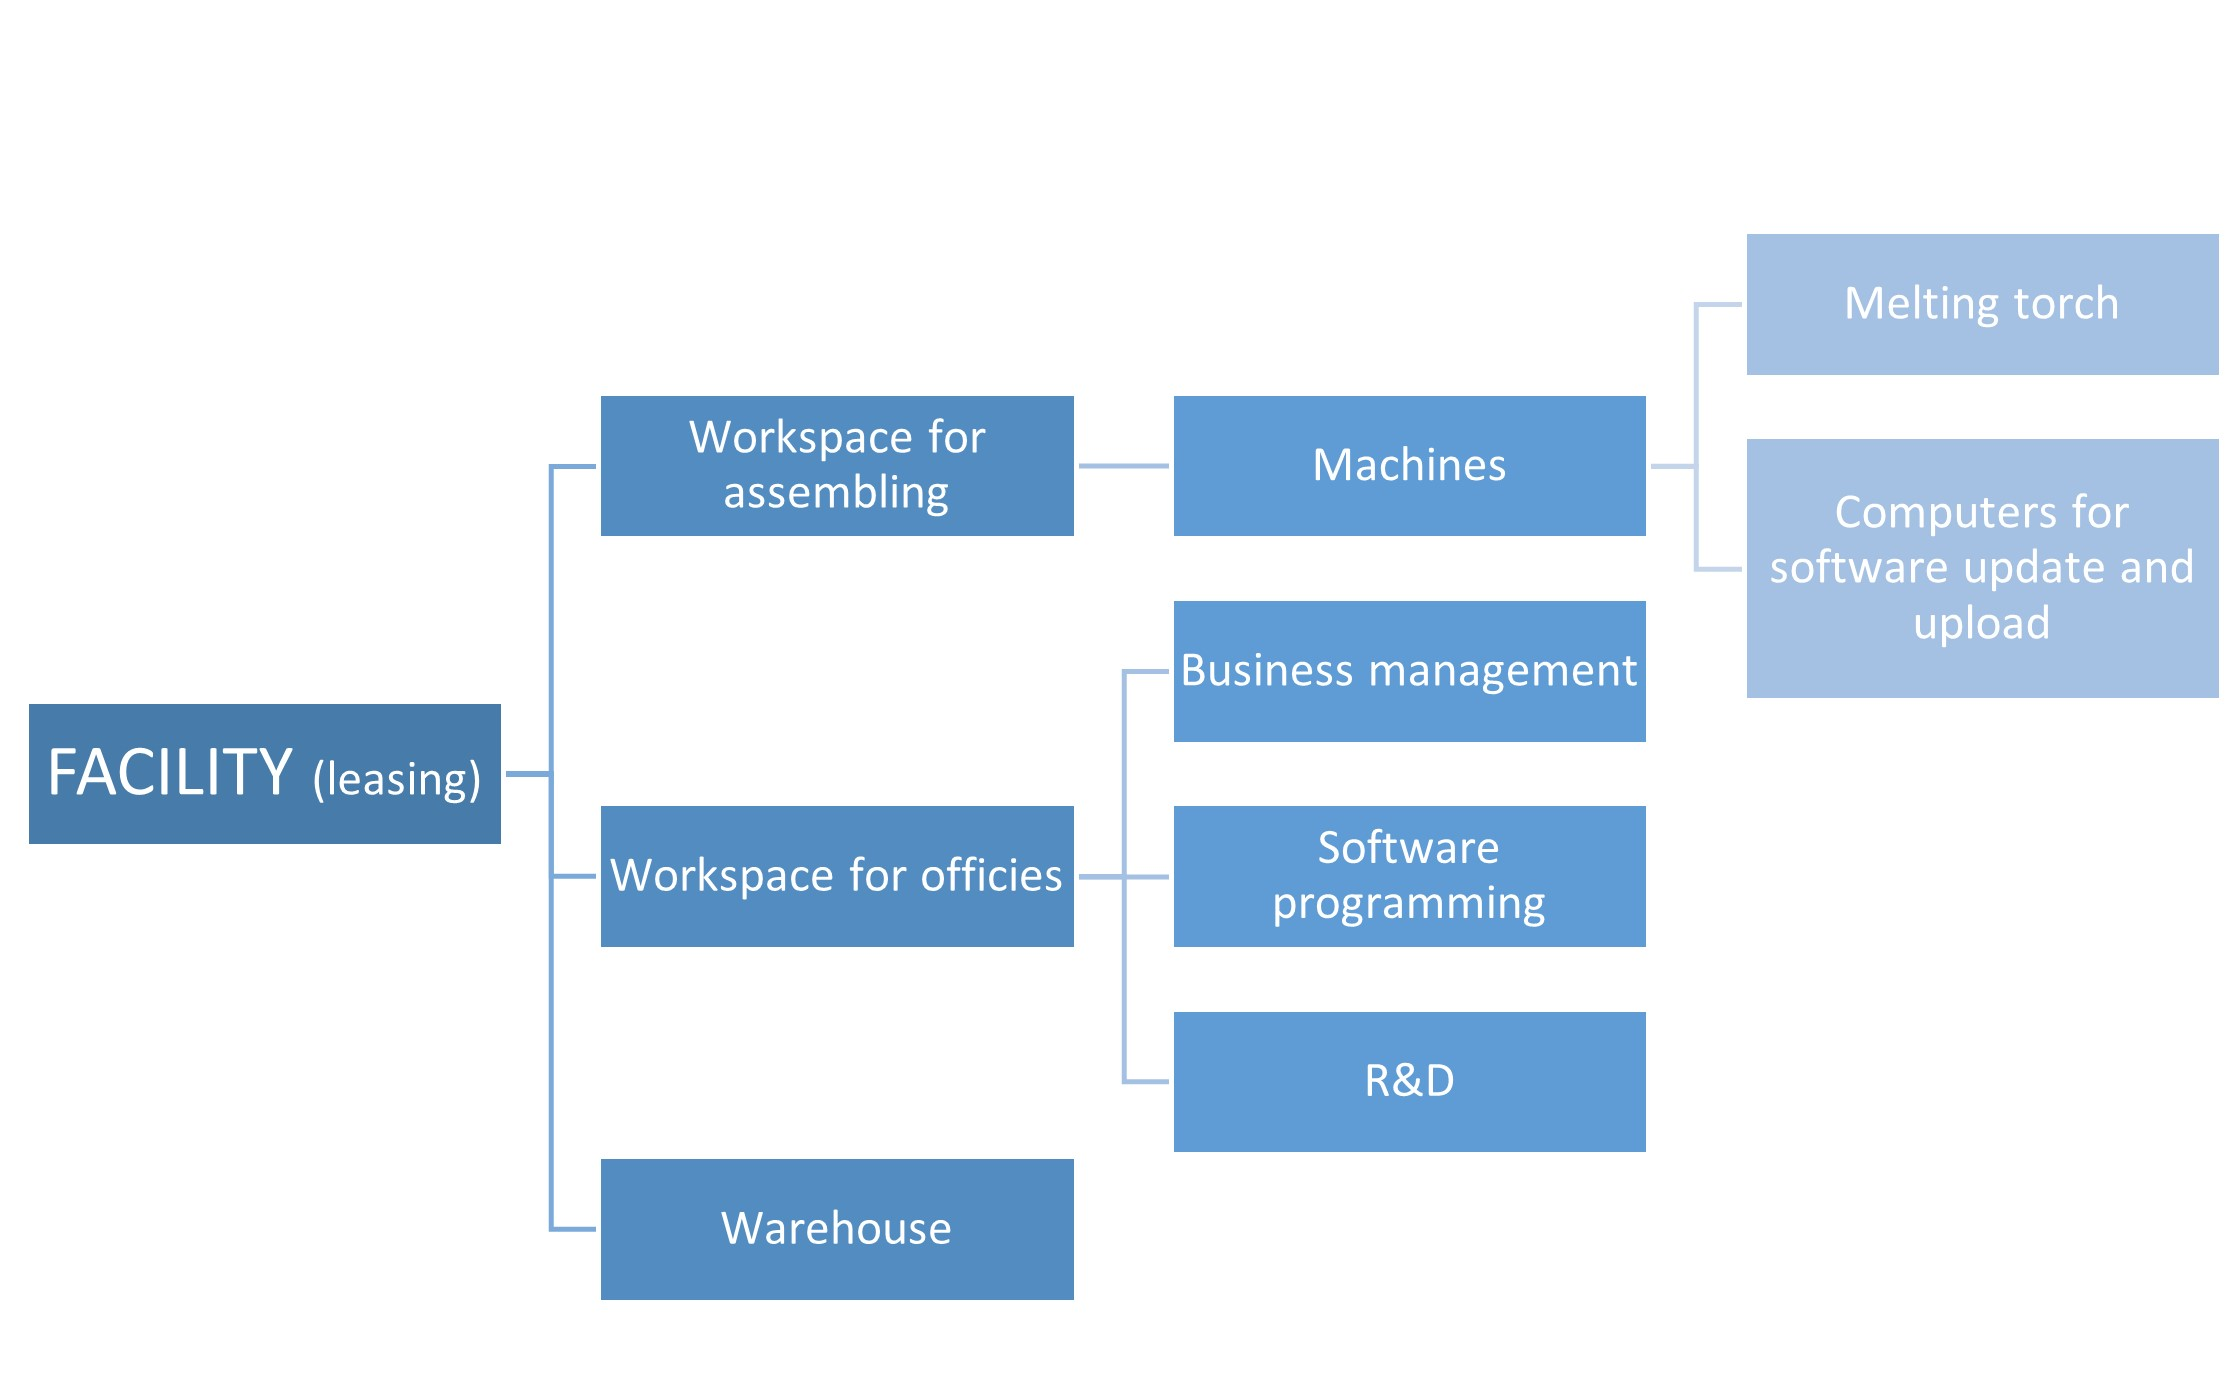
\includegraphics[width=1\textwidth]{images/Facility.jpg}
\caption{Facility}
\end{figure}
\subsection{Operations Strategy And Plans}
Our main business strategy is to subcontract all the production of basic pieces to some partner company. The reason for this choice is to maintain costs sufficiently low for the very start of our society in order to survive the most difficult years. As a matter of fact, machines have a high cost that a newborn society cannot afford. So, our approach will be to buy manufactured components and then assemble them in our facility. In future years maybe we will expand, and we will produce our own components indoors.

\subsection{Development Status And Tasks: Milestones}
The objective our society has is to be fully operative by the end of the next year. The company will be born in January 2021. The very first period will be devoted to the design of the BottAll and to set up the structure of the company. Once we have finished the development of the product, we will take some time in order to prototype and test it. This period is crucial because as the bottle will be tested, we will also conduct a campaign of crowdfunding in order to realize forward steps.
As soon as we earn enough money from the crowdfunding campaign, we will focus on the leasing of the facility where the company will work. Our purpose is to find the right place by at most the end of the summer of 2021. During this period, we will also be looking for partners to produce the components. However, contracts will be stipulated only after the facility has been found.
We think we will be able to start the production of the BottAll by the last months of the year. Luckily, by the start of September, the first bottles will be finished. During this period, we would like also to finish the design of our website where the bottles will be sold in the future months.
By the end of the year our product will be on the market ready to satisfy many customers.
From 2022 onward we will also look for some key partnership with popular brand companies who might want a personalized product to sold with their brand on.\\ 
% Please add the following required packages to your document preamble:
% \usepackage[table,xcdraw]{xcolor}
% If you use beamer only pass "xcolor=table" option, i.e. \documentclass[xcolor=table]{beamer}
\begin{table}[H]
\centering
\begin{tabular}{l|l}
\toprule
\multicolumn{1}{c|}{January-February 2021} & \begin{tabular}[c]{@{}l@{}}-Development and design of the product\\ -Setting up company's board structure\end{tabular} \\ \hline
March-April 2021                                                    & \begin{tabular}[c]{@{}l@{}}-Prototyping\\ -Crowdfunding\end{tabular}                                                   \\ \hline
May-June-July 2021                                                  & -Facility leasing                                                                                                      \\ \hline
July-August 2021                                                    & -Finding partners for manufacturing                                                                                    \\ \hline
September 2021                                                      & -Start of the production                                                                                               \\ \hline
November 2021                                                       & -Go to market                                                                                                          \\ \hline
2022 onward                                                         & -Future partnership with some popular brands                                                                           \\ \bottomrule
\end{tabular}
\caption{Milestones}
\end{table}


\subsection{Challenges And Risks}
The main risks for the company are that in the process there could be some delays in some specific sections of the production. These delays may be due to our internal society as for example some issues with the programming of the website or of the product itself, while other issues can also be due to the suppliers which can have delays in their production and so, we will have no components to keep the production going.
